
\documentclass[10pt]{article}
\usepackage[utf8]{inputenc}
\usepackage{graphicx}
\usepackage{amsmath, amssymb}
\usepackage{geometry}
\usepackage{caption} 
\geometry{a4paper, margin=0.5in, landscape} 

\begin{document}

\section*{Comparative EIS Kinetics Report}
\textbf{Model Structure:} \texttt{R0-p(R1-p(R2,CPE2),CPE1)} \\
\textbf{Used data:} altered data, first 2 points removed and points with $freq > 2e+04$ removed

\begin{center}
    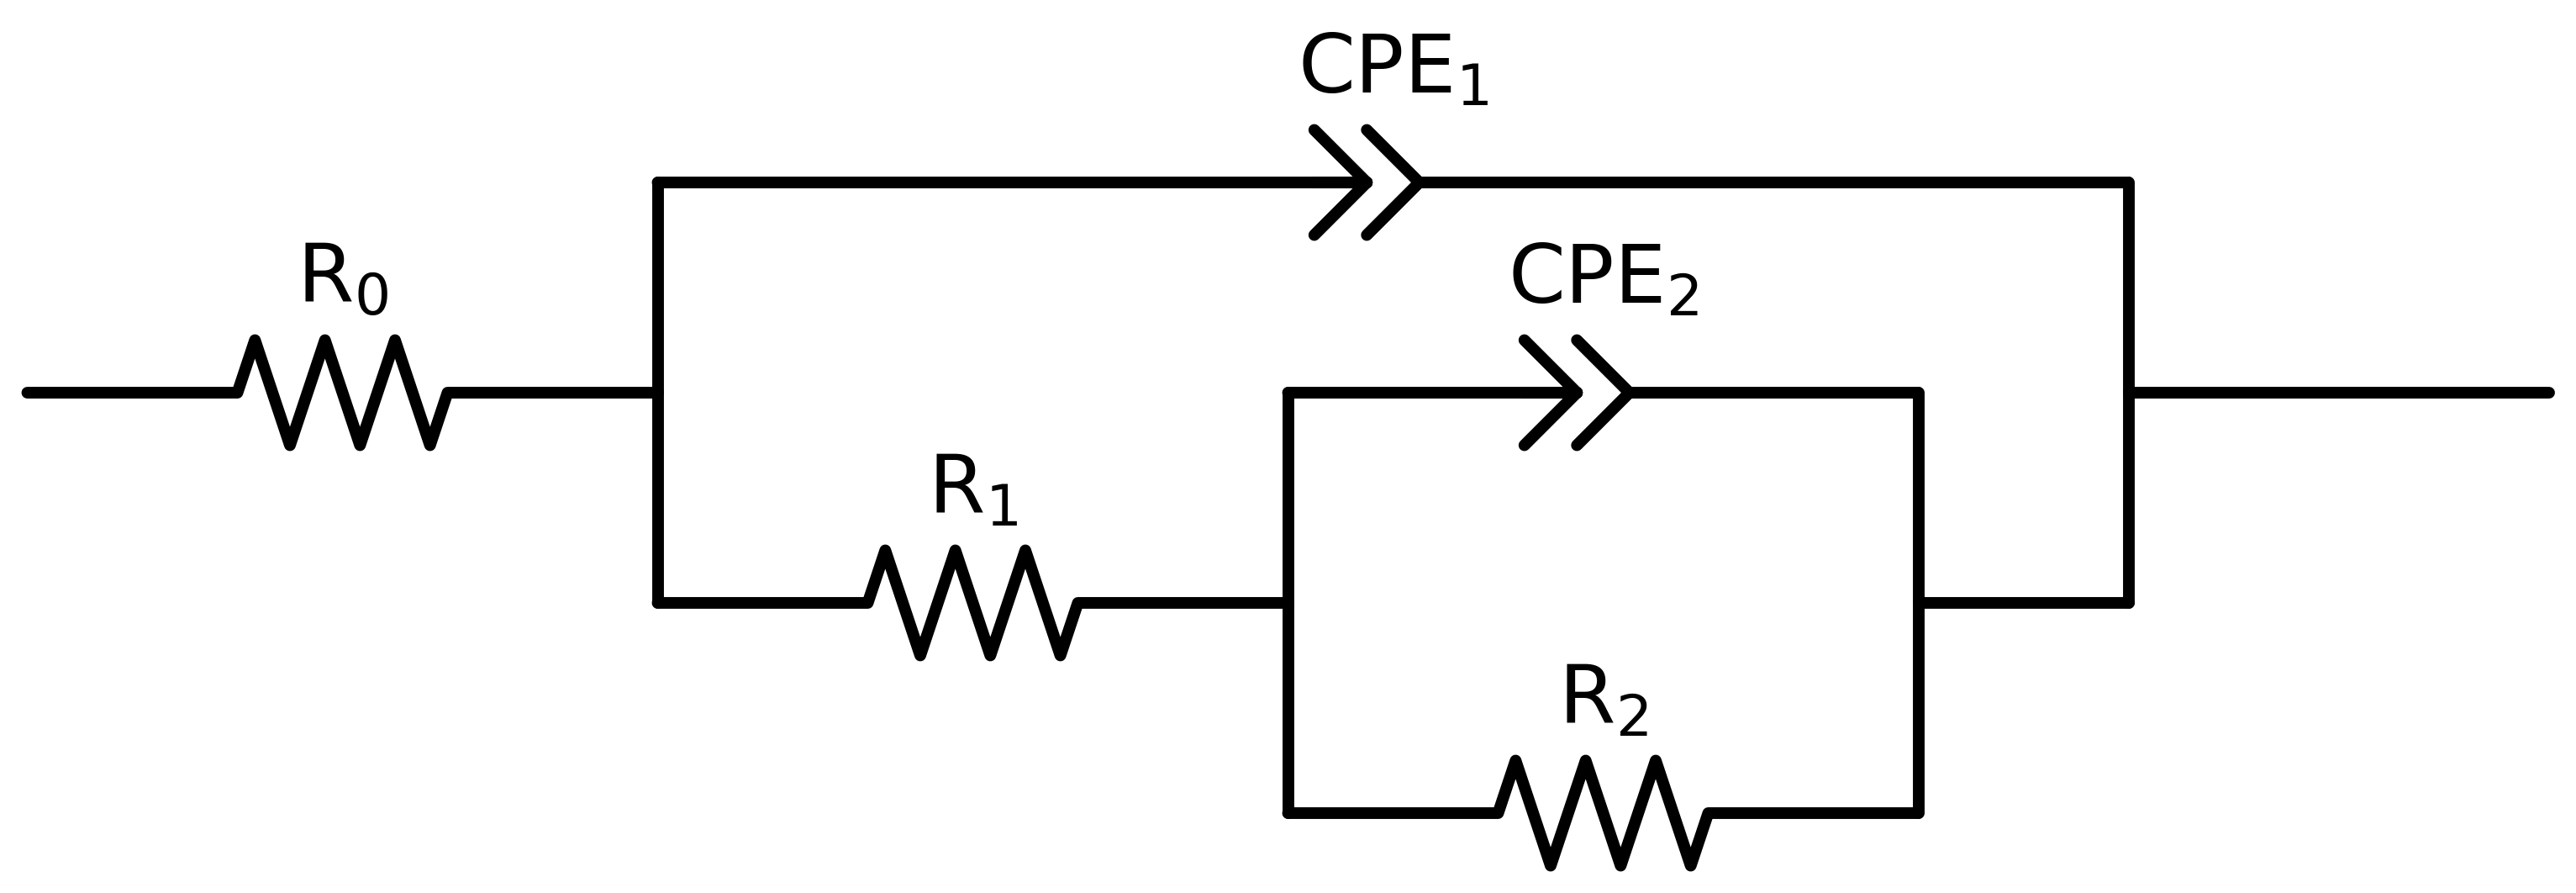
\includegraphics[width=0.45\textwidth]{../../2RC.png}
\end{center}

\renewcommand{\arraystretch}{1.6} 
\begin{table}[h!]
    \centering
    \footnotesize
    \begin{tabular}{|l|c|c|c|c|c|c|}
        \hline
        \textbf{Element} & \textbf{Unit} & \textbf{Bounds} & \textbf{Cauvel\_3\_BTA\_24H} & \textbf{Cauvel\_3\_BTA\_48H} & \textbf{Cauvel\_3\_BTA\_72H} & \textbf{Cauvel\_3\_BTA\_168H} \\ \hline
        $R_{0}$ & $\Omega$ & $[1.0e-03, 1.0e+03]$ & $8.01e+01 \pm 4.2e-01$ & $8.32e+01 \pm 4.2e-01$ & $8.75e+01 \pm 3.8e-01$ & $6.13e+01 \pm 5.1e+00$ \\ \hline
        $R_{1}$ & $\Omega$ & $[1.0e+00, 1.0e+08]$ & $1.36e+04 \pm 1.1e+03$ & $7.83e+03 \pm 2.9e+02$ & $7.35e+03 \pm 1.8e+02$ & $4.14e+01 \pm 9.4e+00$ \\ \hline
        $R_{2}$ & $\Omega$ & $[1.0e+00, 1.0e+08]$ & $5.04e+04 \pm 1.2e+03$ & $4.42e+04 \pm 6.3e+02$ & $3.49e+04 \pm 5.0e+02$ & $3.59e+04 \pm 3.2e+03$ \\ \hline
        $Q_{2}$ & $\Omega$$^{-1}$ sec$^{a}$ & $[1.0e-11, 1.0e-03]$ & $6.46e-06 \pm 3.2e-07$ & $2.26e-05 \pm 3.2e-07$ & $3.91e-05 \pm 4.6e-07$ & $2.49e-06 \pm 1.0e-06$ \\ \hline
        $n_{2}$ & - & $[5.0e-01, 1.0e+00]$ & $9.67e-01 \pm 2.3e-02$ & $8.21e-01 \pm 1.0e-02$ & $7.92e-01 \pm 9.3e-03$ & $1.00e+00 \pm 4.3e-02$ \\ \hline
        $Q_{1}$ & $\Omega$$^{-1}$ sec$^{a}$ & $[1.0e-11, 1.0e-03]$ & $1.34e-05 \pm 3.1e-07$ & $1.12e-05 \pm 2.3e-07$ & $1.07e-05 \pm 1.8e-07$ & $5.89e-05 \pm 2.2e-06$ \\ \hline
        $n_{1}$ & - & $[5.0e-01, 1.0e+00]$ & $8.51e-01 \pm 3.4e-03$ & $8.66e-01 \pm 3.1e-03$ & $8.68e-01 \pm 2.6e-03$ & $5.00e-01 \pm 2.4e-02$ \\ \hline
        \textbf{$\chi^2$} & - & -  & $2.819e-04$ & $2.745e-04$ & $2.272e-04$ & $4.858e-03$ \\ \hline

    \end{tabular}
\end{table}


\newpage
\section*{Analysis Results: 24H}
\begin{center}
    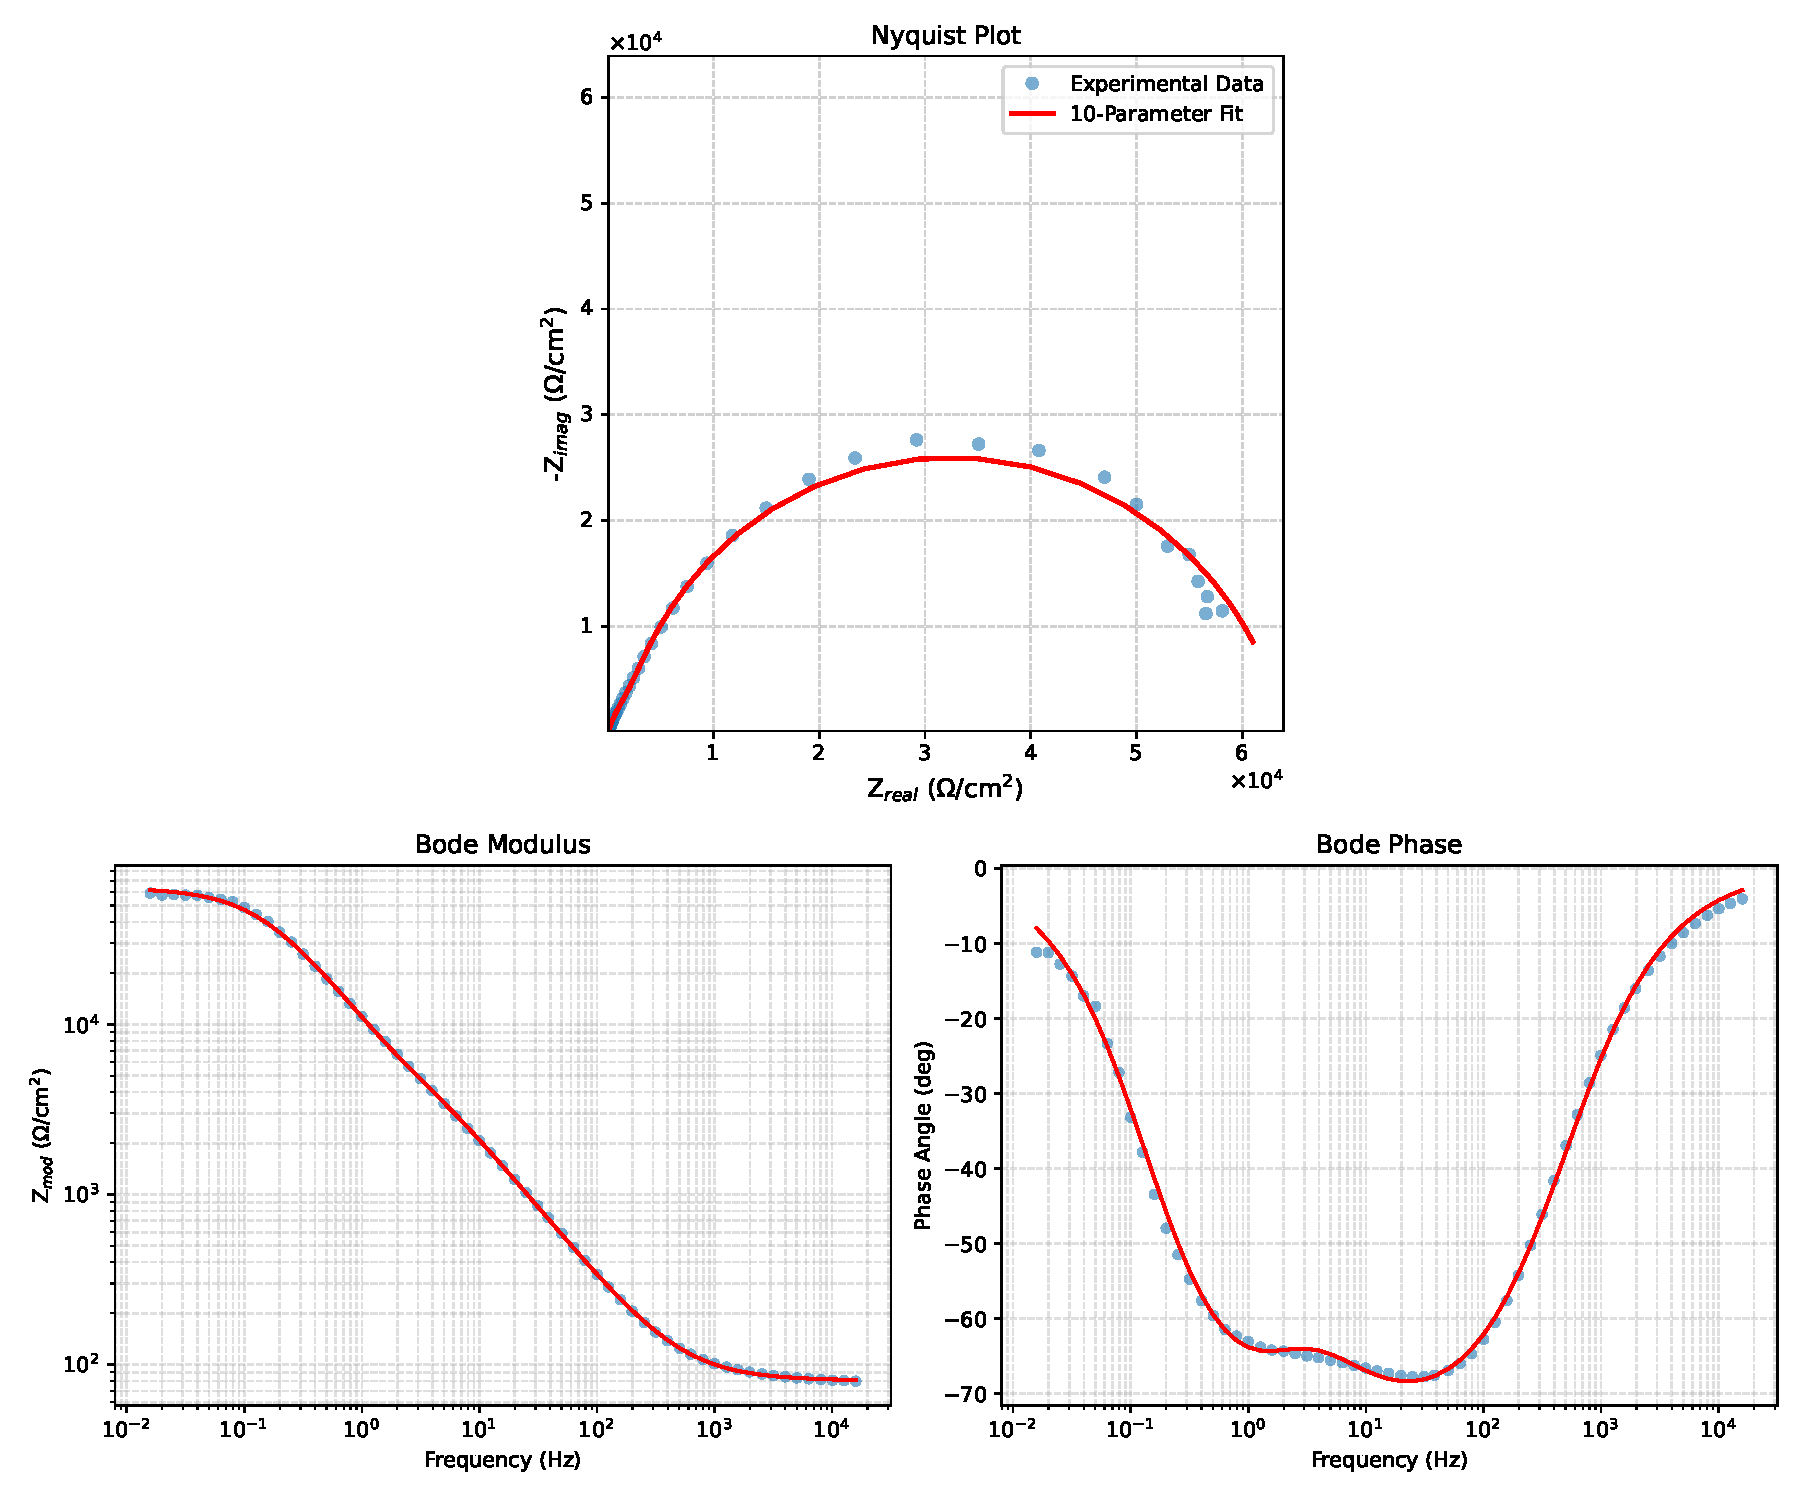
\includegraphics[width=0.7\textwidth]{plots_Cauvel_3_BTA_24H_2RC_1.pdf}
    \captionof{figure}{EIS Fit Results for Cauvel\_3\_BTA\_24H}
\end{center}

\newpage
\section*{Analysis Results: 48H}
\begin{center}
    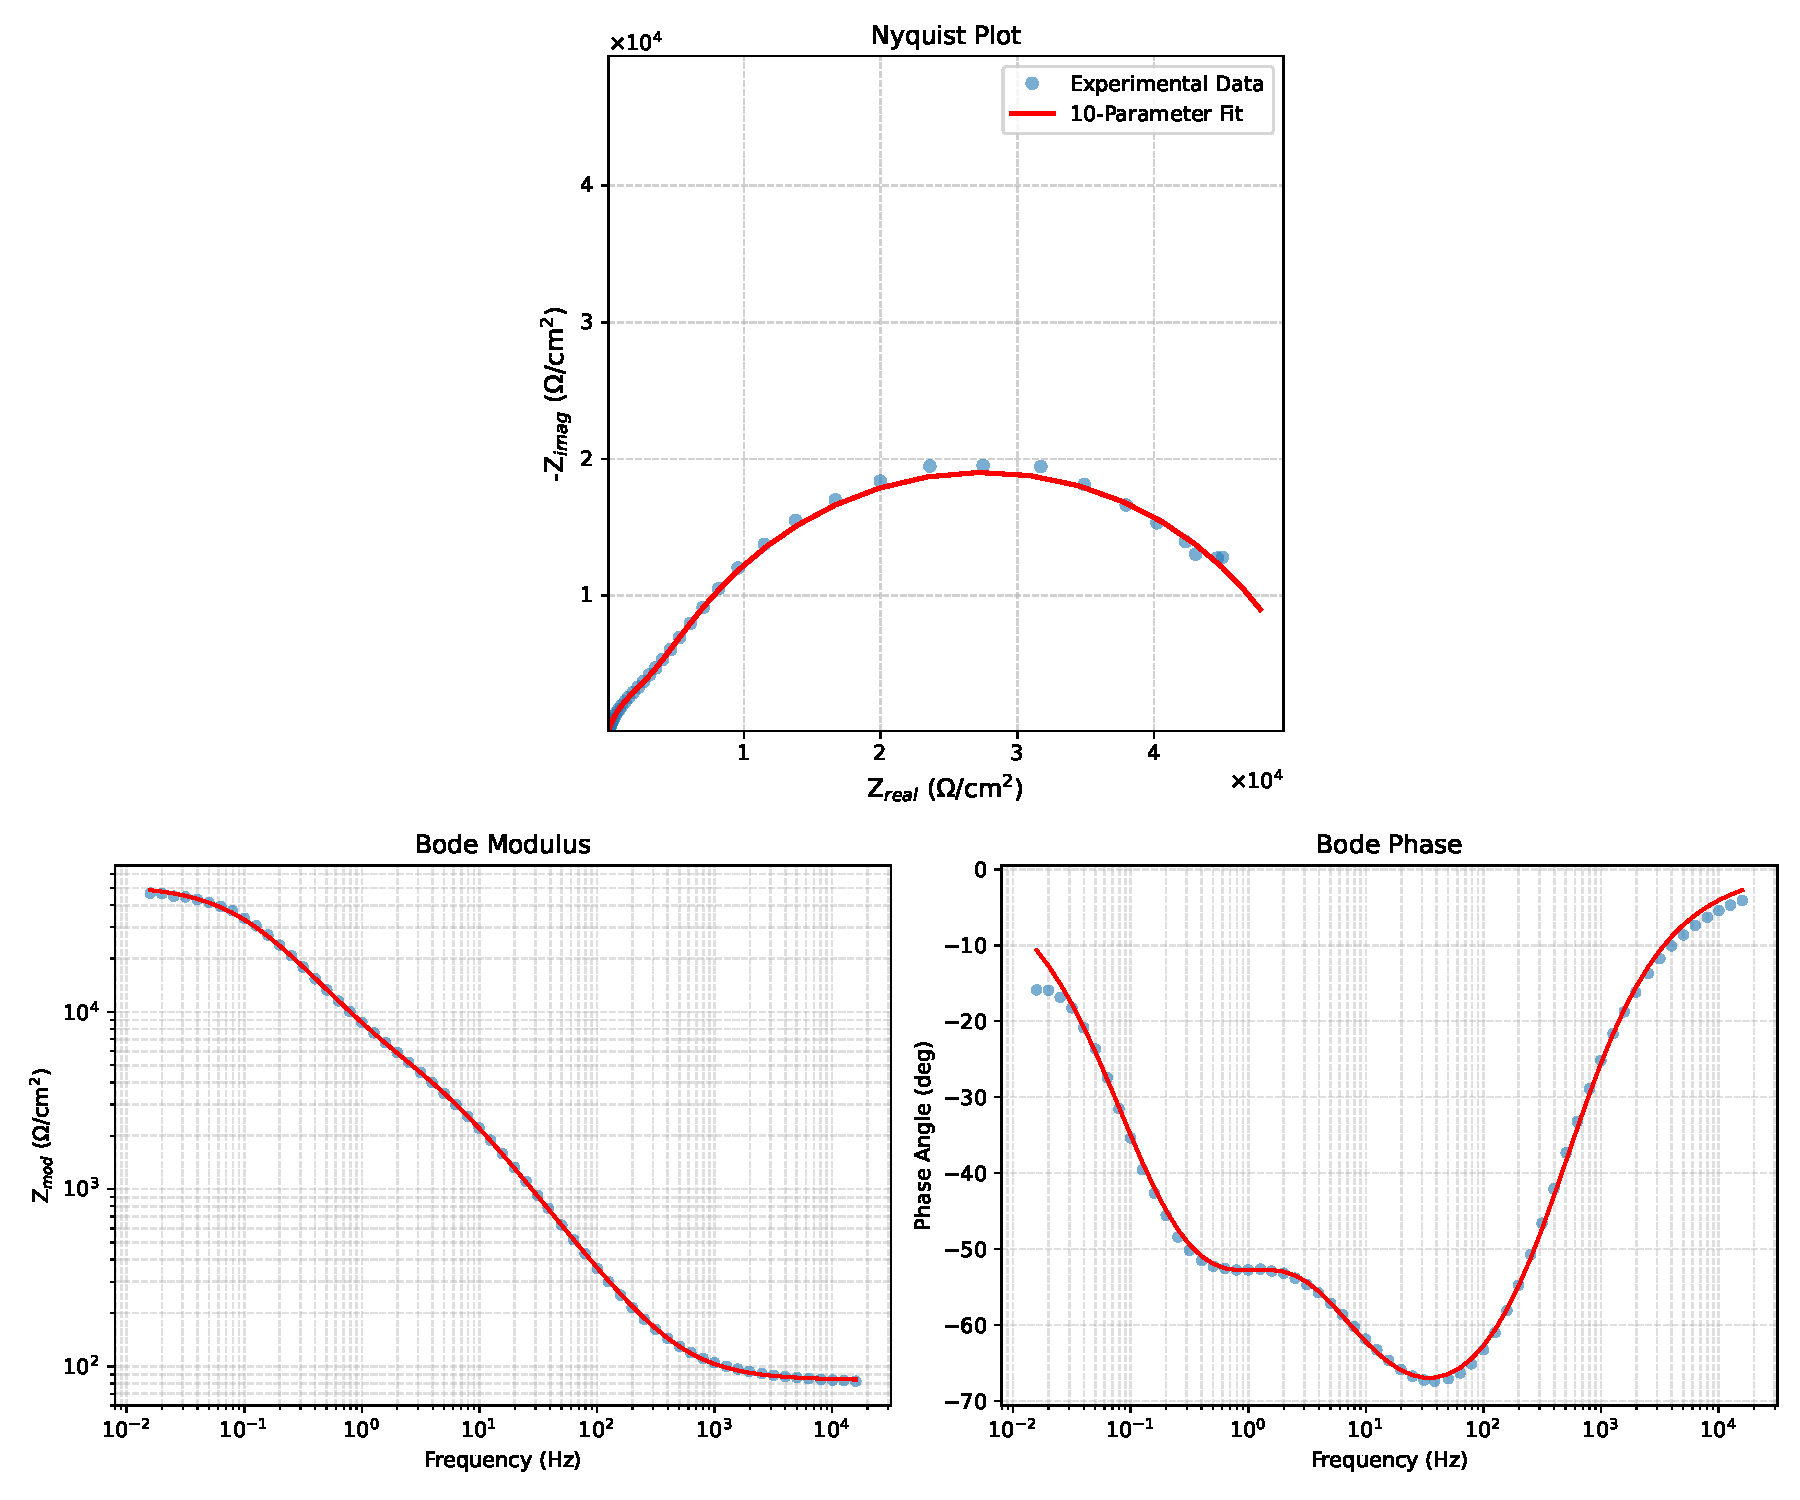
\includegraphics[width=0.7\textwidth]{plots_Cauvel_3_BTA_48H_2RC_1.pdf}
    \captionof{figure}{EIS Fit Results for Cauvel\_3\_BTA\_48H}
\end{center}

\newpage
\section*{Analysis Results: 72H}
\begin{center}
    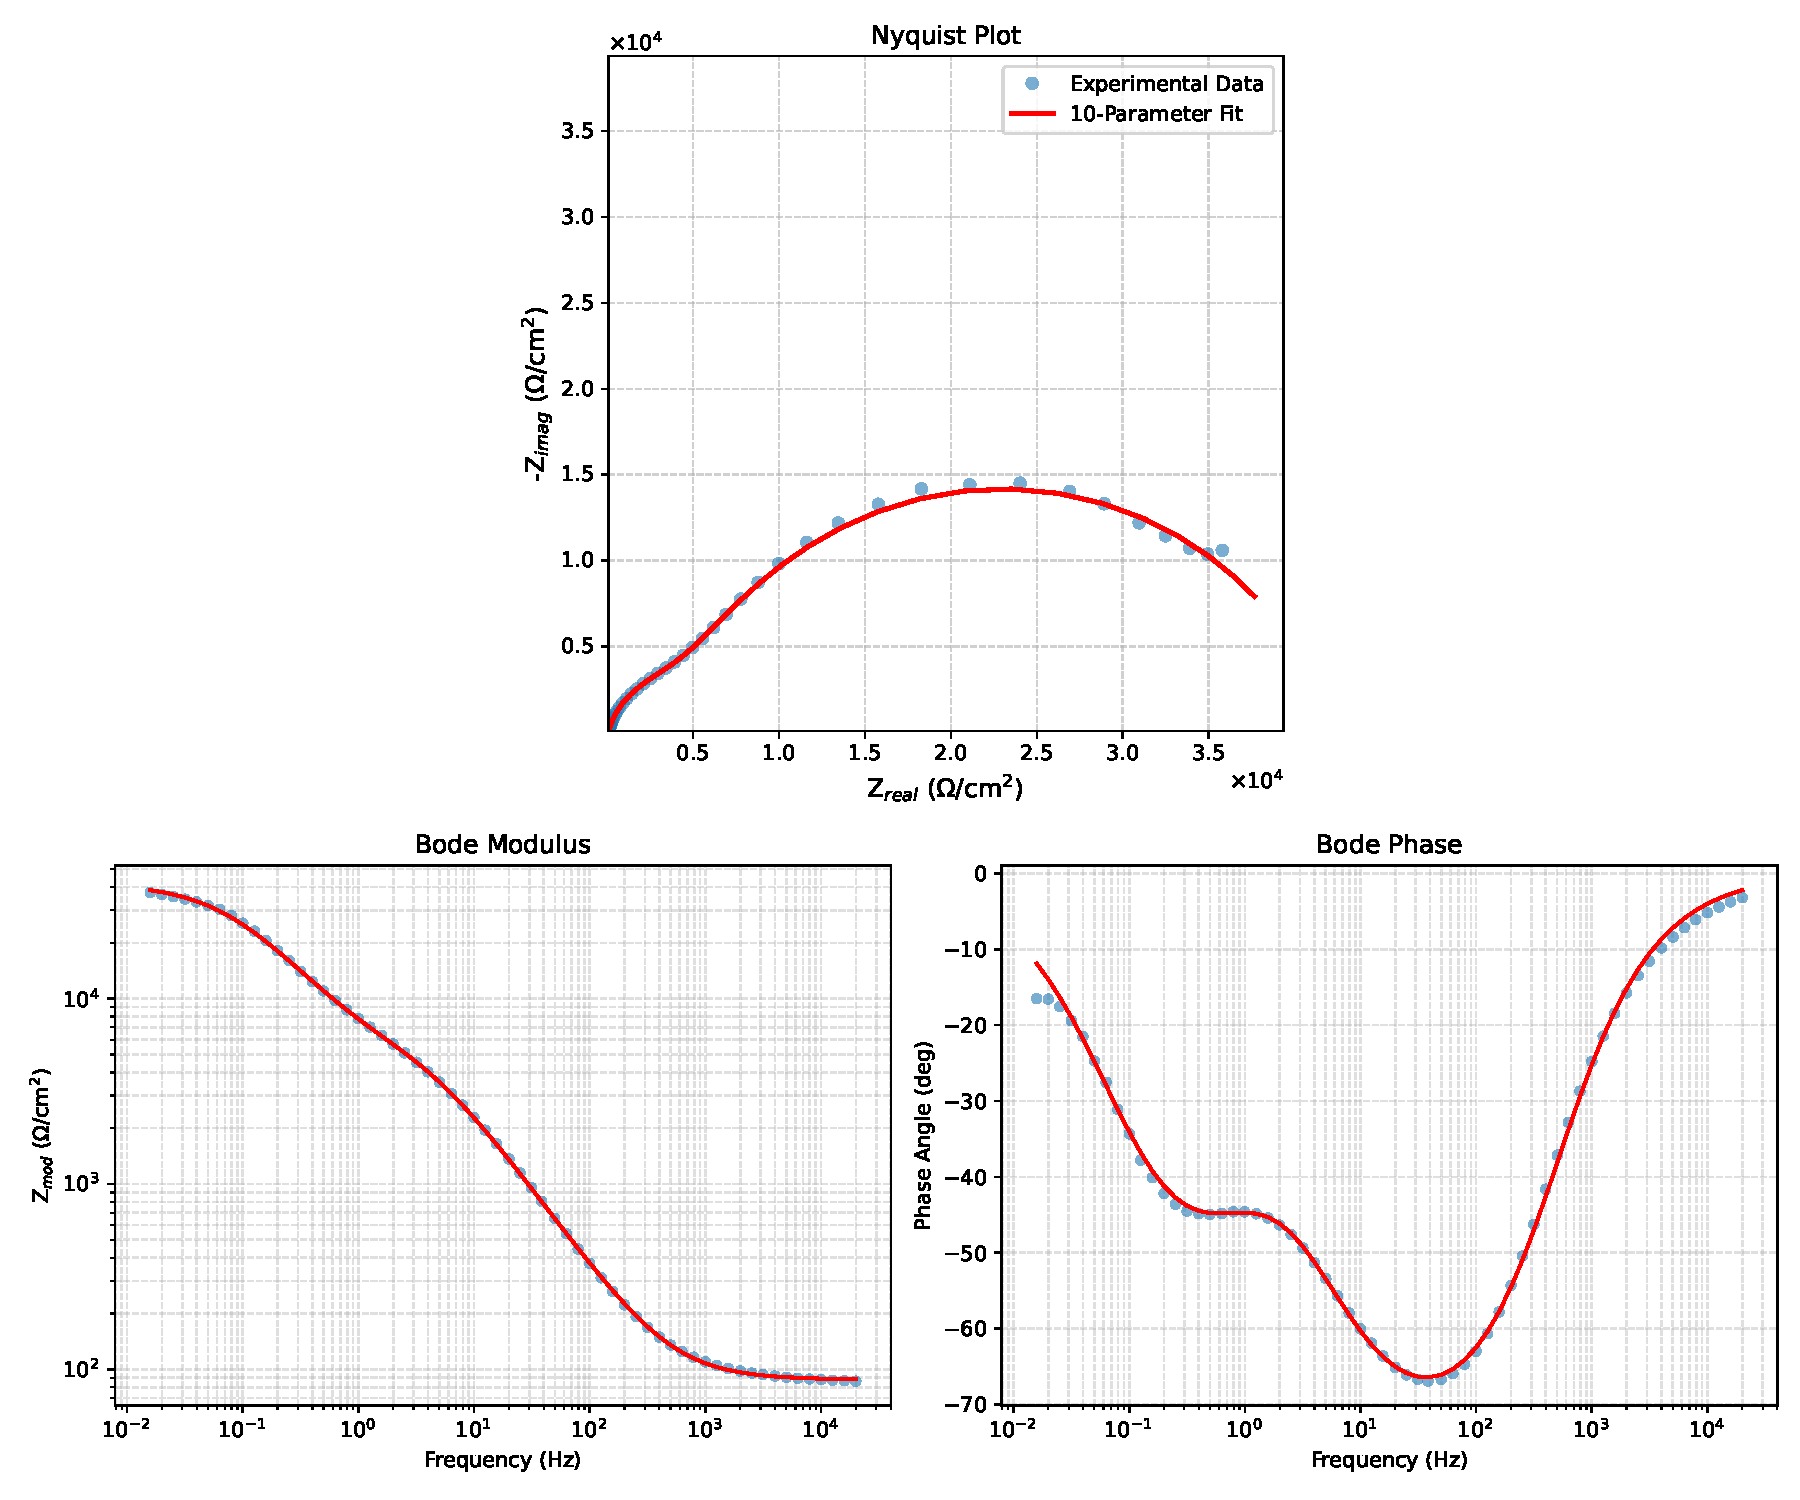
\includegraphics[width=0.7\textwidth]{plots_Cauvel_3_BTA_72H_2RC_1.pdf}
    \captionof{figure}{EIS Fit Results for Cauvel\_3\_BTA\_72H}
\end{center}

\newpage
\section*{Analysis Results: 168H}
\begin{center}
    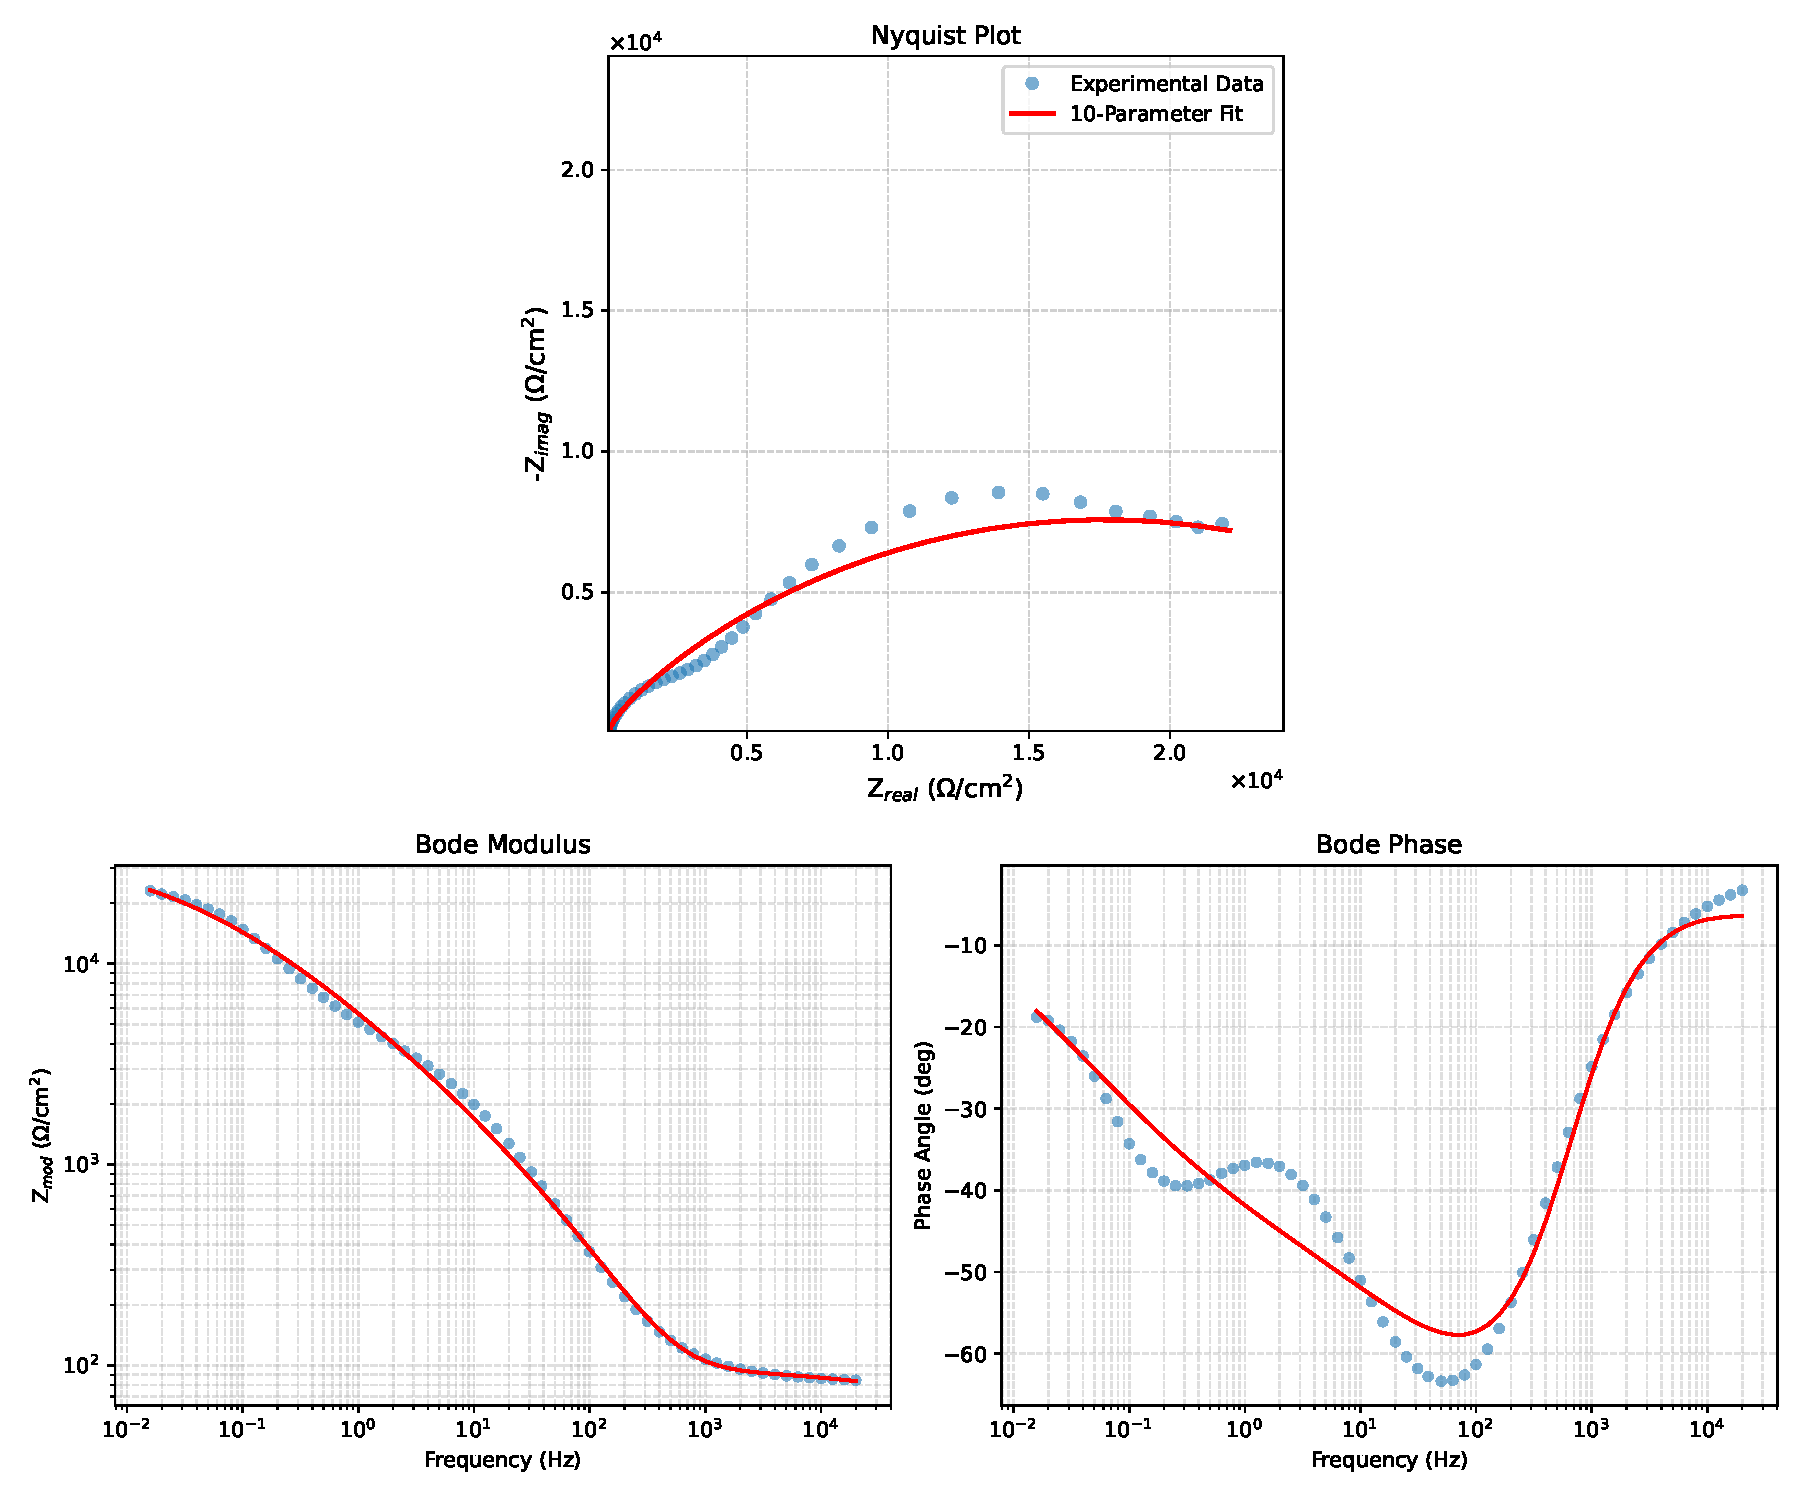
\includegraphics[width=0.7\textwidth]{plots_Cauvel_3_BTA_168H_2RC_1.pdf}
    \captionof{figure}{EIS Fit Results for Cauvel\_3\_BTA\_168H}
\end{center}


\end{document}
